\subsection{Browse data in the PCDB: The `Data viewer' window}\label{subsec_data_viewer} 
Figure \ref{fig_pgadmin3_data_viewer_country} displayes the window that pops-up when selecting the country table in the \texttt{config\_data} schema in of the \texttt{polconfdb} database on the CMS database server.

\begin{figure}[ht!]
\centering
  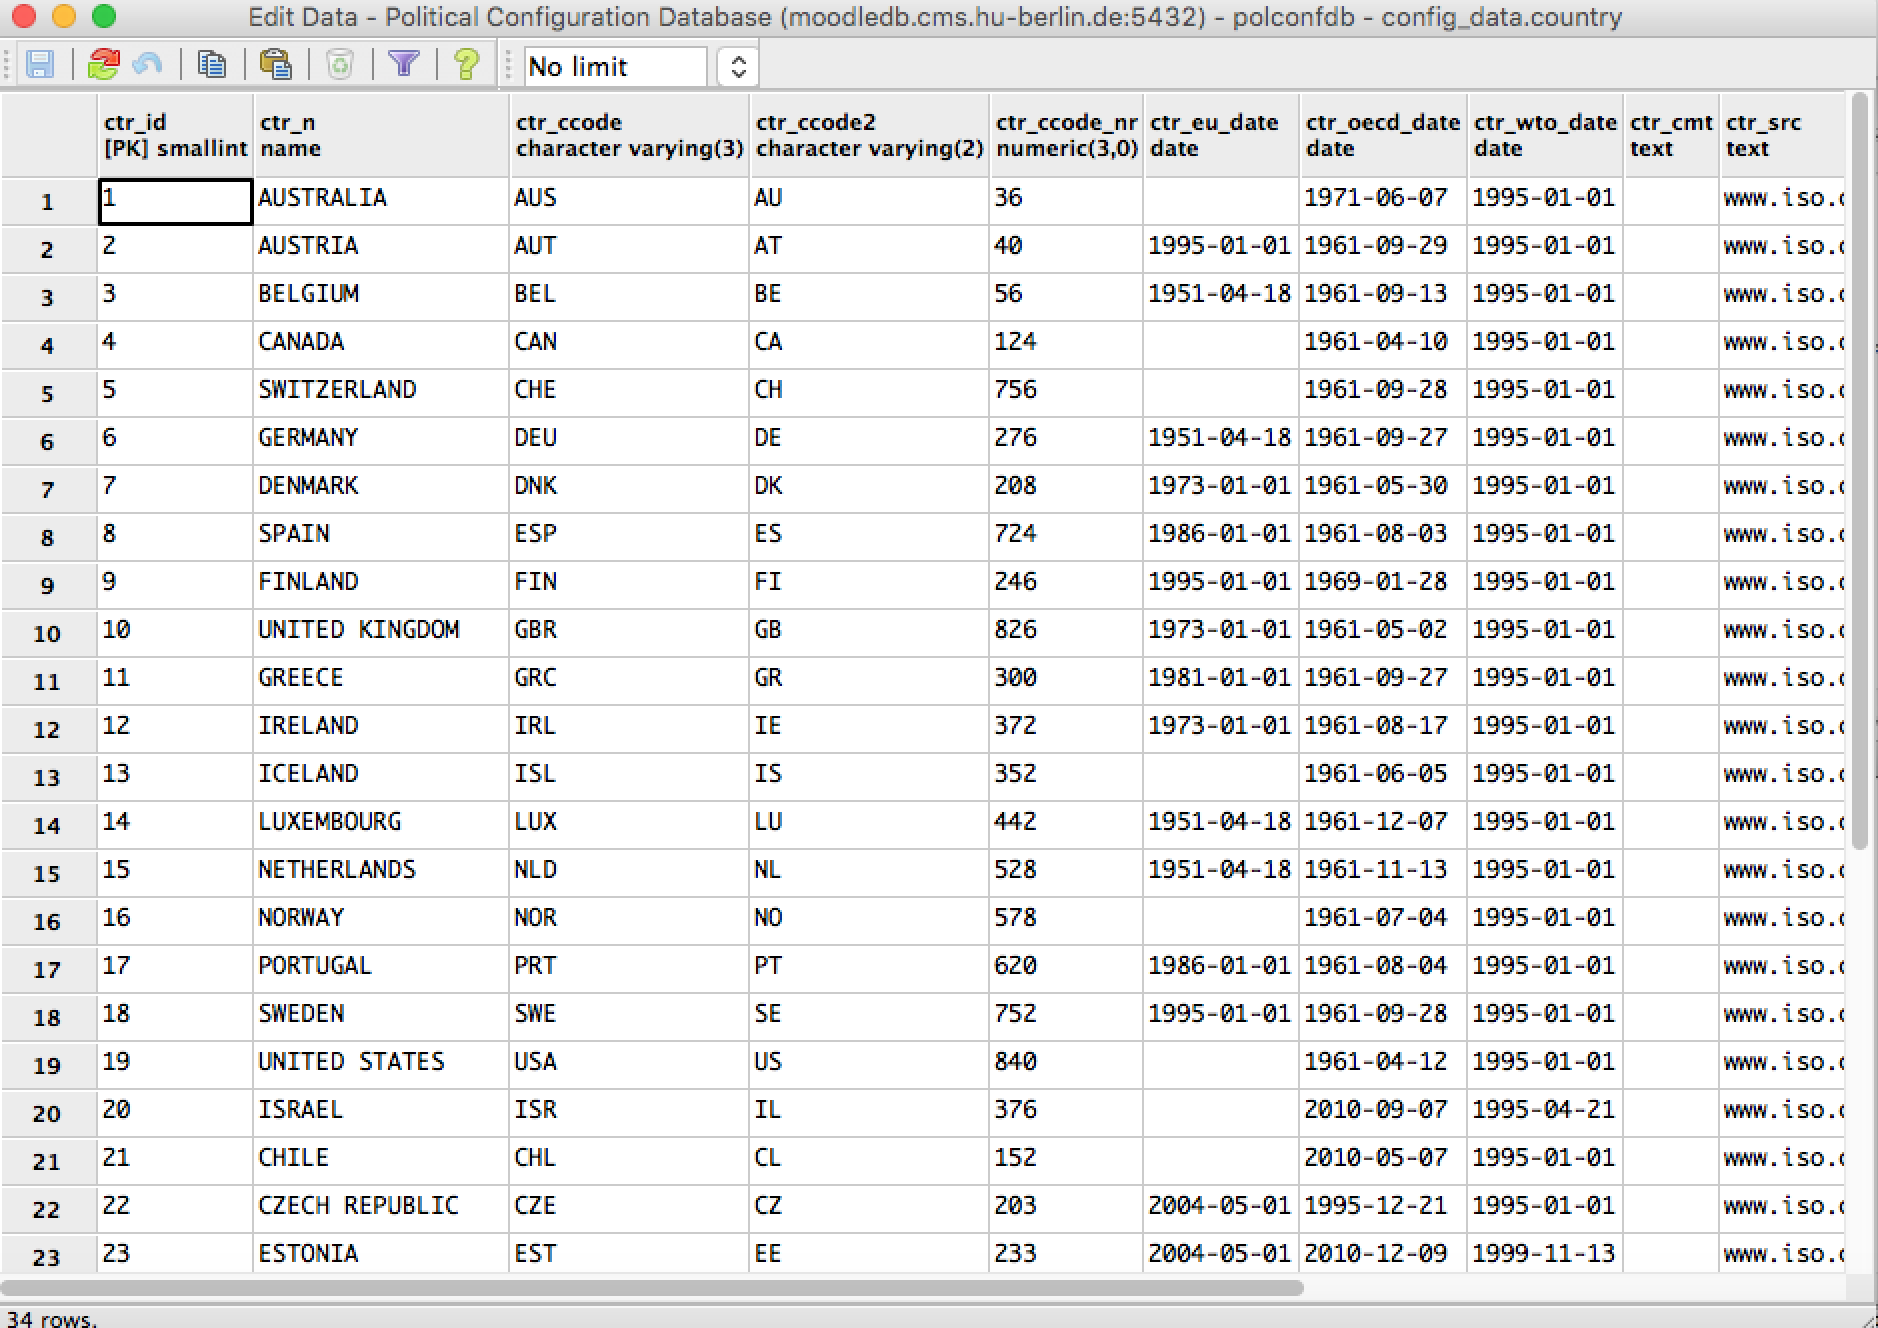
\includegraphics[width=.8\textwidth,trim= 0 0 0 0, clip]{pcdb_documentation_screenshots/pgadmin3_data_viewer_country.png}
    \caption{Data Viewer pop-up window of country table in \texttt{config\_data} schema.}
    \label{fig_pgadmin3_data_viewer_country}
\end{figure}

The `Data viewer' window has the following elements (from top to bottom):
\begin{itemize}
\item[-] The {\bf window header} informs you that this is an editor (i.e., if writing-rights are granted to your role, you can edit the data by double-clicking inside cells and change their content), and about the name of the server you are connected to (here ``Political Configuration Database''), the host and port number (``(moodledb.cms.hu-berlin.de:5432)''), as well as the database (``polconfdb''), and schema and table names (``config\_data.country''). This is in fact the all information you need to know which data table is displayed.

\item[-] The window's {\bf tool bar} allows you to refresh the current data table (icon with one red and one green circular arrow); and, in case you have writing rights, to save changes (blue shaded disc icon), or undo changes to the data (right-to-left upward-bend blue shaded arrow). 

\item[-] The {\bf main panel} displays the data of the selected table or view. 
Columns are variables, where the main panel's header displays variable names and types (e.g., \texttt{ctr\_id} and \texttt{smallint}), and contraints are displayed in square brackets (e.g., \texttt{[PK]}, which stands for primary key).
By default, all rows are listed; but you can limit the number of rows displayed in the most-right tool bar panel by typing a number in the input window label `No limit' by default.) 

\item[-] The {\bf window footer} informs you how many rows the displayed data has.
\end{itemize}
